\documentclass{article}

\usepackage{graphicx}
\usepackage{tikz}
\usepackage{tikzsymbols}
\usetikzlibrary{calc,patterns,shapes.geometric}
\pagestyle{empty}
\usepackage[margin=0pt]{geometry}
\geometry{papersize={14in,12in}}

\def\centerarc[#1](#2)(#3:#4:#5){\draw[#1] ($(#2)+({#5*cos(#3)},{#5*sin(#3)})$) arc (#3:#4:#5);}

\begin{document}
	\begin{figure}
		\centering
		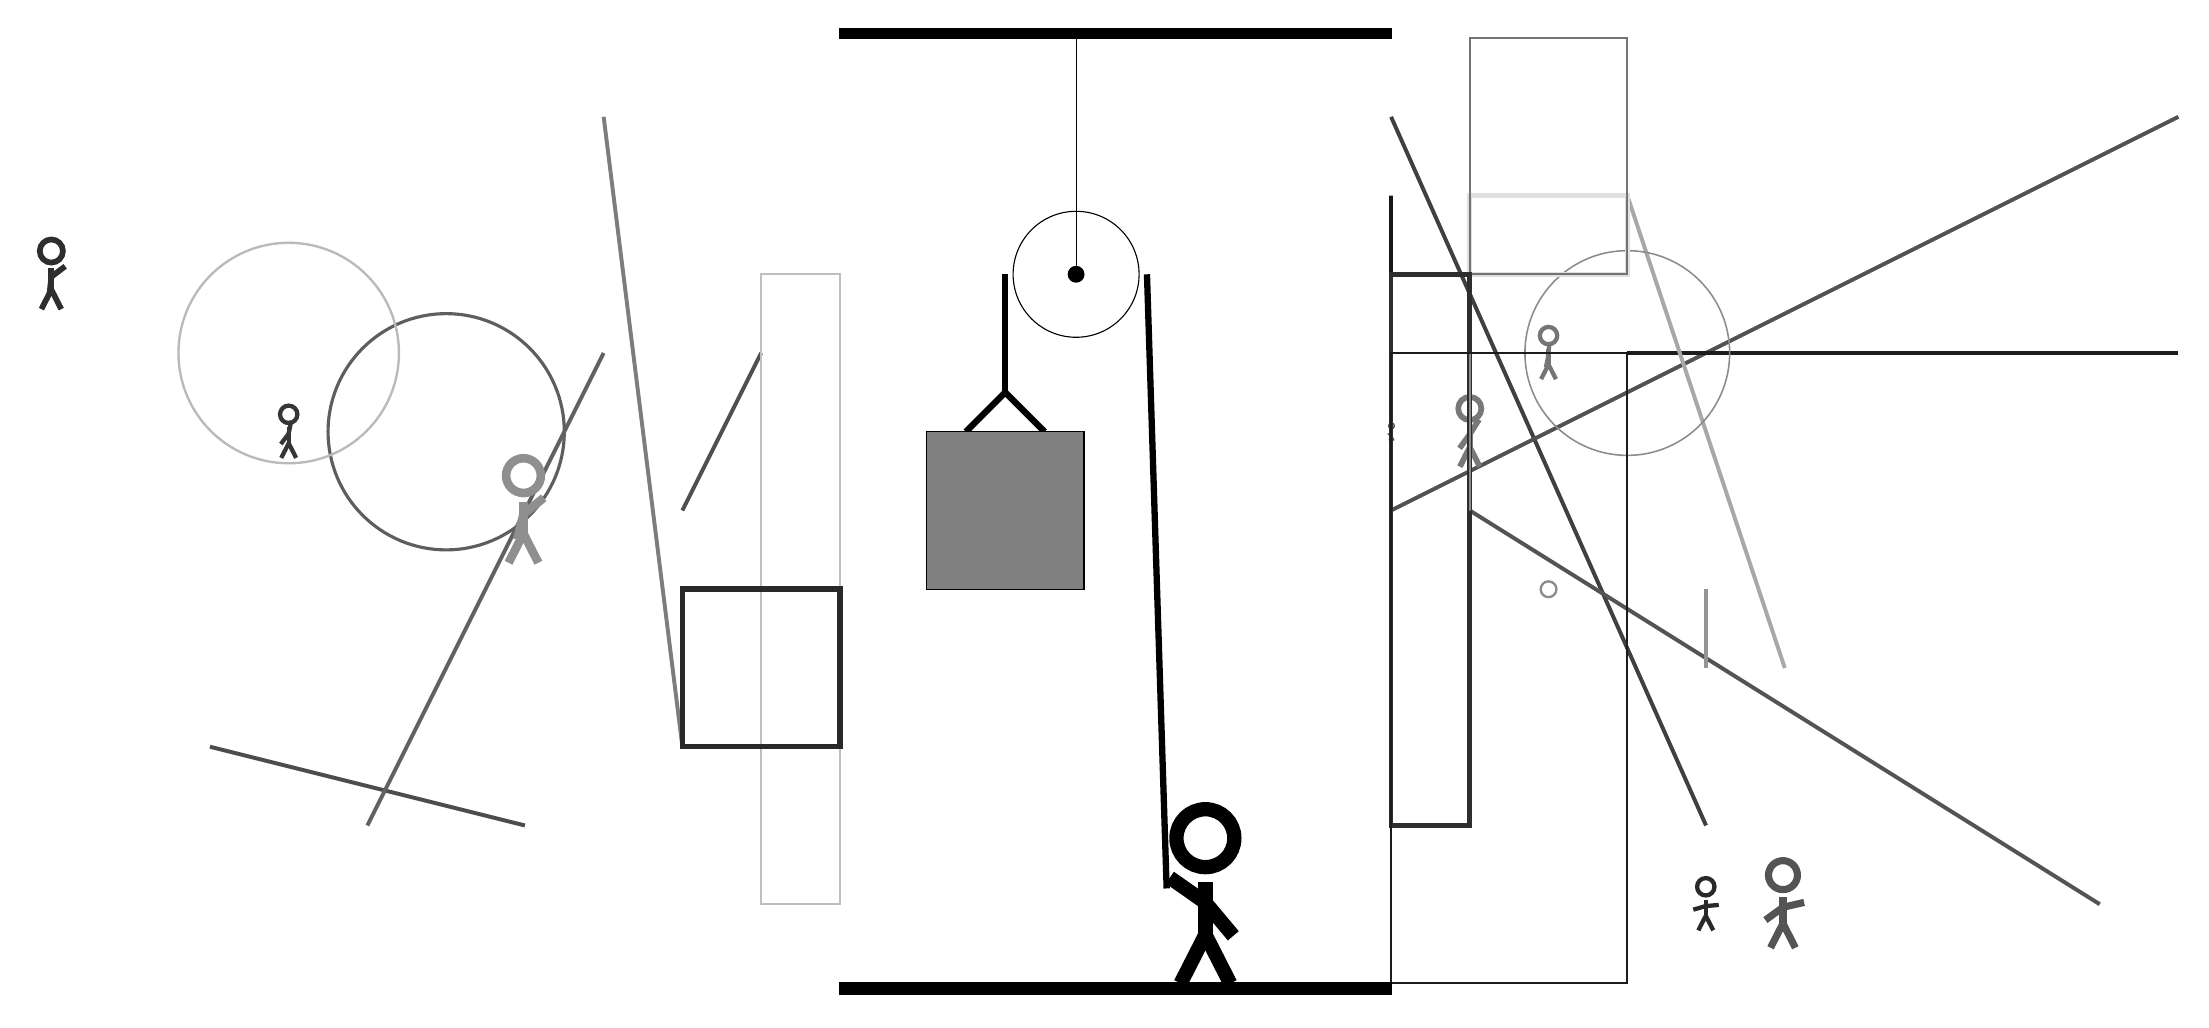
\begin{tikzpicture}
			%%%%% START %%%%%
			
			\draw[fill=black] (-2, 9) rectangle (5, 9.125);
			
			\draw (1, 6) circle (0.8);
			\draw[fill=black] (1, 6) circle (0.1);
			\draw (1, 9) -- (1, 6);
			
			\draw[line width=0.8mm] (-0.4, 4.0) -- (0.1, 4.5) -- (0.6, 4.0);
			\draw[fill=black!50] (-0.9, 4.0) rectangle (1.1, 2.0);
			
			\draw[line width=0.8mm] (0.1, 6) -- (0.1, 4.5);
			\centerarc[line width=0.8mm](1, 6)(0:180:0.9);
			\draw[line width=0.8mm](1.9, 6) -- (2.15, -1.8);
			
			\node at (2.6, -1.9) {\Strichmaxerl[10][-35][-50]};
			
			\draw[line width=0.5mm, color=black!75](9, -1) -- (5, 8);
			
			\draw[line width=0.5mm, color=black!68](5, 3) -- (15, 8);
			\draw[line width=0.2mm, color=black!75] (-4, 2) rectangle (-3, 0);
			\node[line width=0.3mm, color=black!53] at (6, 4) {\Strichmaxerl[4][54][58]};
			
			\draw[line width=0.5mm, color=black!89](8, 5) -- (15, 5);
			
			\node[line width=0.3mm, color=black!66] at (5, 4) {\Strichmaxerl[1][30][78]};
			\draw[line width=0.5mm, color=black!34](10, 1) -- (8, 7);
			\node[line width=0.5mm, color=black!67] at (10, -2) {\Strichmaxerl[5][36][13]};
			\draw[line width=0.5mm, color=black!67](6, 3) -- (14, -2);
			\draw[line width=0.5mm, color=black!70](-6, -1) -- (-10, 0);
			\node[line width=0.4mm, color=black!54] at (7, 5) {\Strichmaxerl[3][78][87]};
			\draw [line width=0.4mm, color=black!63](-7, 4) circle (1.5);
			\draw[line width=0.4mm, color=black!91] (5, 5) rectangle (5, 7);
			
			\draw [line width=0.2mm, color=black!45](8, 5) circle (1.3);
			\draw [line width=0.3mm, color=black!27](-9, 5) circle (1.4);
			\draw[line width=0.5mm, color=black!69](-3, 5) -- (-4, 3);
			\draw[line width=0.6mm, color=black!12] (6, 7) rectangle (8, 6);
			\draw[line width=0.5mm, color=black!51](-5, 8) -- (-4, 0);
			\draw[line width=0.5mm, color=black!62](-5, 5) -- (-8, -1);
			\draw[line width=0.3mm, color=black!25] (-3, 6) rectangle (-2, -2);
			\draw [line width=0.3mm, color=black!45](7, 2) circle (0.1);
			\draw[line width=0.3mm, color=black!55] (6, 9) rectangle (8, 6);
			\draw[line width=0.5mm, color=black!42](9, 1) -- (9, 2);
			\node[line width=0.3mm, color=black!82] at (-12, 6) {\Strichmaxerl[4][84][37]};
			\node[line width=0.3mm, color=black!84] at (9, -2) {\Strichmaxerl[3][16][5]};
			\draw[line width=0.6mm, color=black!82] (5, -1) rectangle (6, 6);
			\node[line width=0.7mm, color=black!44] at (-6, 3) {\Strichmaxerl[6][76][39]};
			\draw[line width=0.3mm, color=black!46] (6, 3) rectangle (6, 5);
			
			\draw[line width=0.7mm, color=black!84] (-2, 2) rectangle (-4, 0);
			\node[line width=0.3mm, color=black!79] at (-9, 4) {\Strichmaxerl[3][53][79]};
			\draw[line width=0.3mm, color=black!89] (5, -3) rectangle (8, 5);
			
			
			\draw[fill=black] (-2, -3) rectangle (5, -3.15);
			
			%%%%% END %%%%%
		\end{tikzpicture}
	\end{figure}	
\end{document}